

\section{Color and time evolution}\label{sec:timegaps}

\begin{center}

\begin{figure}[t!]
\centering 
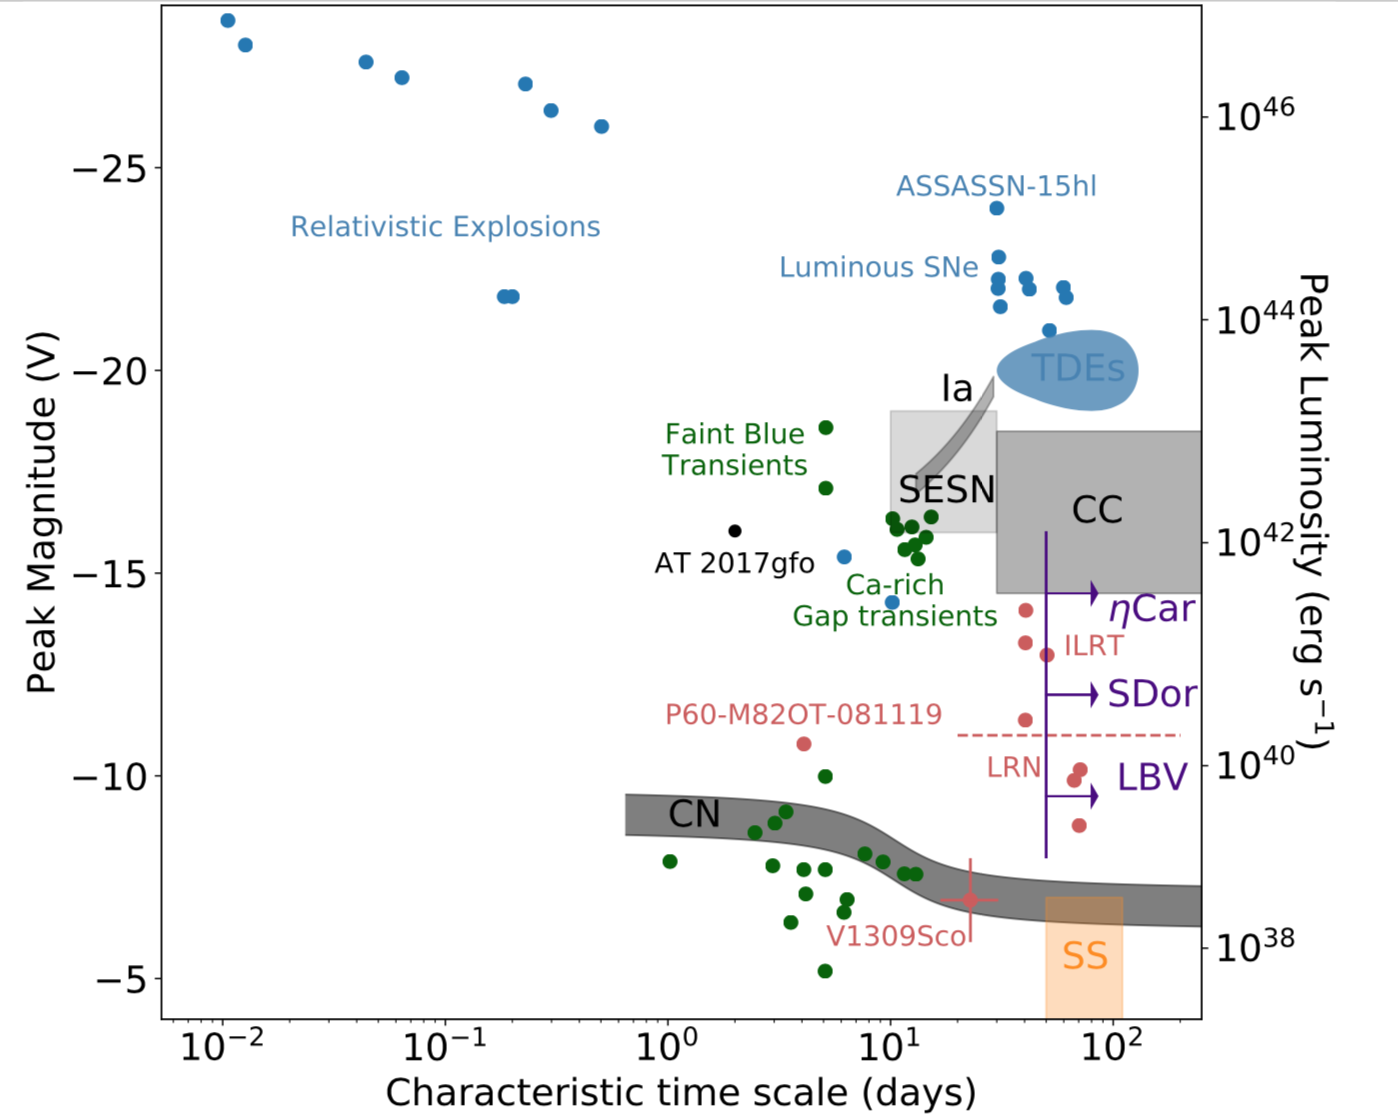
\includegraphics[scale=0.4]{figures/taumv_updated_wgap_lr.png}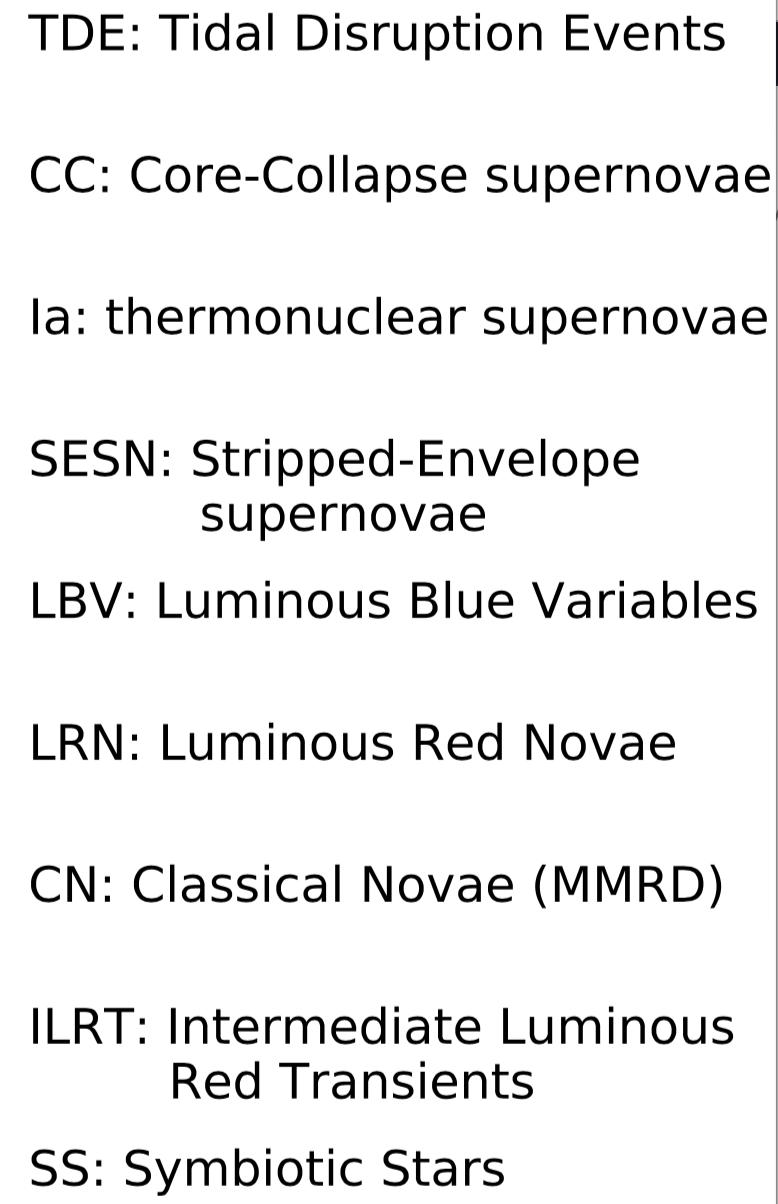
\includegraphics[scale=0.3]{figures/taumv_updated_legend.png}
\caption{The phase space of transients, reproduced with modifications and permission from \citet{lsst}: the intrinsic brightness is plotted against the characteristic time scale of evolution. Shaded areas indicate the  region of this phase-space occupied by various classes of objects and individual objects are indicated for some of the the less numerous classes. The notable gap at all intrinsic magnitudes fainter than -20 is likely due, at least in part, to an observational bias as surveys are typically not able to probe large volumes of the Universe at short time down to faint brightnesses. }
\label{fig:phasespace}
\end{figure}
\end{center}

Astrophysical transients and variable phenomenon captured humanity's curiosity through the history of science. Modern astrophysics and particularly the use of digital equipment in the last half-century enabled extremely fast paced advances in this field. Figure \ref{fig:phasespace}, reproduced from \citet{lsst}, shows the phase space of known astrophysical transients: transients and variable phenomena occupy different regions of this phase space of intrinsic brightness \emph{vs} characteristic time scales. At the beginning of the 20th century, essentially only supernovae were known to exist, and the phase space populated rapidly with many different classes of transients since then. It is worth noting the gap on the left of $\sim 1~\mathrm{day}$: while it is possible that this region is scarcely populated {\it intrinsically}, it is also true that an observational bias impairs discovery in this region:  to be effective in discovery and characterization surveys  need to reach high depth and high cadence simultaneously, while also surveying a large volume if phenomena in this region of the phase space are truly rare.




% time gaps distribution
\begin{figure}[t!]
\centering
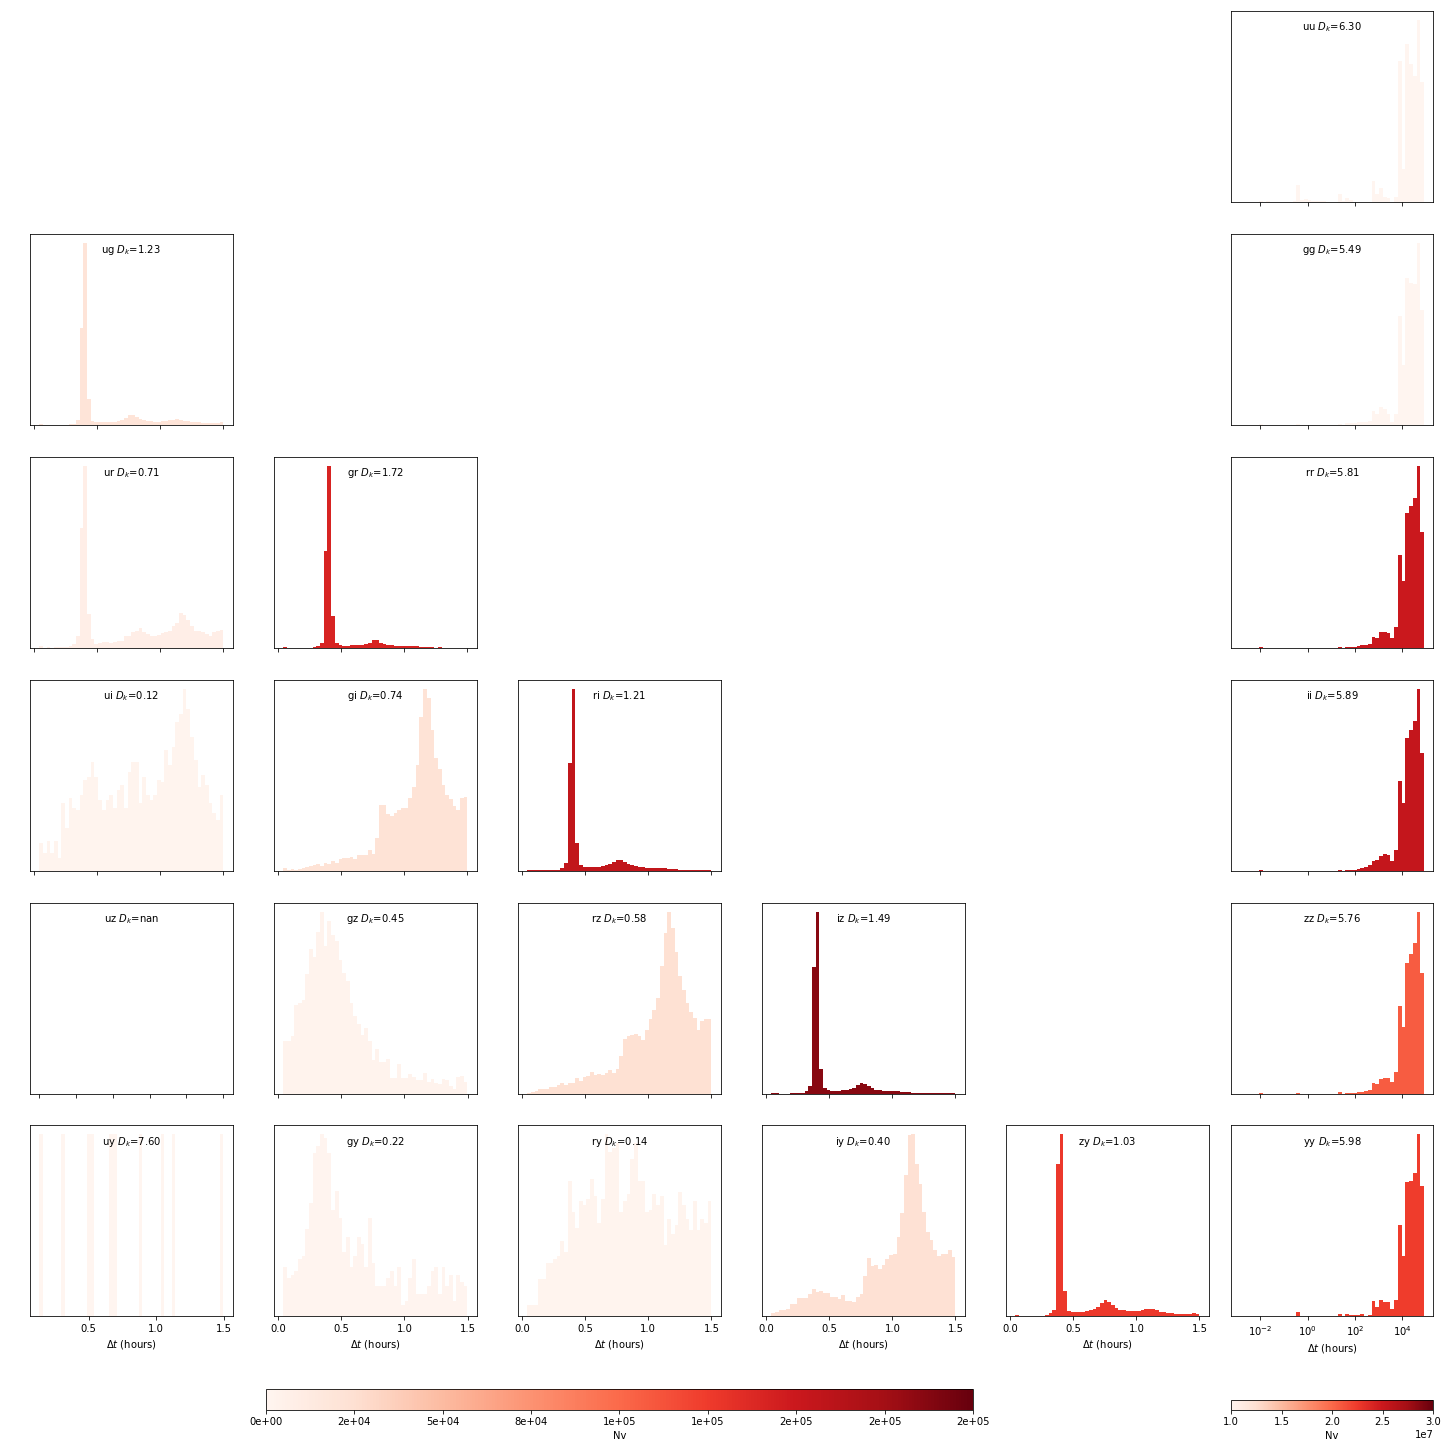
\includegraphics[scale=0.3]{figures/tgaps_hist.png}
\caption{
\new{The distribution of all time gaps for the \texttt{baseline v1.4} \opsim~ \question{Xiaolong please add the exact opsim name}. The triangle plot on the left shows all time gaps between different filters (which enable the measurement of color) within 1.5 hours. The column of plots on the right shows the distribution of time gaps in the same filter for the 10-year survey, which enables the measurement of brightness changes. The filters are indicated in each quadrant: from $u$ to $y$ moving from top to bottom and left to right. All histograms are normalized but the intensity of the color is proportional to the to total number of observations in that filter-pair, as indicated by the color bar. In each quadrant the value of $D_{KL}$ is  reported (see \autoref{sec:fom:tgaps}).  \question{We note that the majority of observations are taken with adjacent filters, which gives a narrow leverage on the spectral energy distribution (SED), and less power to measure color. Color is in fact better measured with filter that are more separated in wavelength, for example \emph{g-i} or \emph{r-z}, as described in \citep{Bianco_2019}}}
\question{Xiaolong: labels too small, color gets too faint, change label to $D_{KL}$}}
\label{fig:tGapshist}
\end{figure}

Due to their diversity in time scales, color, and evolution, the study of transients and particularly studies that aspire to discover new transient phenomena, requires dense space \emph{and} time coverage.  
%\question{Sufficiently high astrometric accuracy is also highly desirable in order to identify objects of interest with known (or unknown!) populations. I STILL DONT GET IT}. 
The LSST has both high photometric sensitivity and a large footprint, enabling the surveying of  a large volume of Universe. This provide us tremendous opportunities to study the variable sky. %: if the temporal cadence, then, is adequate \citep{lsstSB}, faint, rare and exotic objects are likely to be discovered. 
The LSST's capability to discover unknown-unknowns transients then largely depend on its observation cadence.

Different phenomena will benefit form different observation strategies because of the different phenomenological expression of their intrinsic physics. To make sure the observation strategies under design maximize  our chances to discover unknown unknowns, we created the {\it filterTGapsMetric}, which evaluates specifically  the ability of LSST's observation strategies to capture information about color and its time evolution at multiple time scales. 


\subsection{The \texttt{filterTGapsMetric}}\label{sec:fom:tgaps}

Rubin LSST will image the sky in six filter bands {\it u, g, r, i, z, y}. The {\it filterTGapsMetric} measures all time gaps between two filters in an \opsim, i.e, {\it ug, gr, ri} and so on. The \texttt{ filterTGapsMetric} Figure of Merit evaluates the coverage of time gaps for each filter-pair. We prefer an observation strategy that minimizes uncovered gaps, allowing the preference to differ for single-filter and for two-filter pairs. For example, assume one object changes its overall brightness across the spectrum within 3 hours. If we do not measure its brightness in at least two filters within this time we will not know what the true color of the object is. Homogeneous coverage within 1.5 hours in 2 filters maximizes our ability to measure color and color changes. Meanwhile, to detect brightness changes at different time scales we would prefer a distribution of time gaps for images in the same filter to be homogeneous in log-space.
%its color from {\it u} to {\it r} within 2 hours, if our cadence has no visits between {\it ur} within this time range, then we will definitely miss this kind of objects. 
%NOTE: this is not exactly how it works: we want the colors measured within 1.5 hours because slower would mean you cant tell if you observe color or lightcurve change. Within 1.5 hours we consider that we are agnostic about when to measure the color, and then diversifying within that range gives us less bias. We need to think about how to write this}

%\new{Following the naming convention of the COSEP, the map of evaluated quantities on a field-by-field basis is called the ``metric'', with the $FoM$ the result of the combination of the metric and any other weightings we impose, over the entire sky to distill the metric into a single scalar.}
%\question{this is described in the erlier section already} 
On a field-by-field basis, for each filter pair, the metric and $FoM$ are evaluated as follows:

\begin{itemize}
    \item select the survey (\emph{e.g.} WFD in this paper) and the observation time range using {\tt sqlconstraint} and slice the sky with HealpixelSlicer (see \autoref{sec:MAF}); 
    \item fetch observation times for each field for all visit in either of the two filters;
    \item perform a element-wise subtraction to get all time gaps;
\end{itemize}
\autoref{fig:tGaps} shows the distribution of time gaps for all filters pairs for the \texttt{baseline v1.4  OpSim} \question{Xiaolong please add the exact opsim name}. 


% KL divergence from uniform
\begin{figure}[t!]
\centering
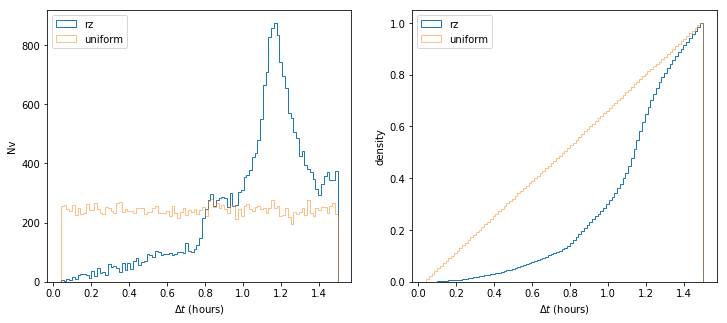
\includegraphics[scale=0.5]{figures/dkl_rz.png}
\caption{
Time gaps in $r-z$ (left) and $??$ (right) from the first year \question{Xiaolong fix the name: baseline operation v1.4} compared to the ``ideal'' distribution, plotted in orange: a uniform distribution for the colors (left) and a uniform distribution in log space for the lightcurve shape (right).  \question{This is not the right plot: we should have $g-i$ on the left and $g-g$ on the right in log scale; labels still too small }}
\label{fig:tGaps}
\end{figure}

% FOM from time gaps
 \begin{figure}[!th]
 \centering
 \gridline{
  \fig{figures/tgapsFOM_0.png}{0.4\textwidth}{(a)} 
  \fig{figures/tgapsFOM_1.png}{0.4\textwidth}{ (b)} 
  }
\caption{Figures of merit ($FoM$) for  75 \opsim~ runs based on the distribution of time gaps. The $FoM$ is calculated as described in Equation \ref{eq:fom:tgaps}. The plot on the \emph{left} shows the $FoM$ for repeat visits in the same filter.  The plot on the \emph{right} shows the value for observations in pairs of different filters. Each \opsim~ is presented as a bar whose length corresponds to the value of the $FoM$. For each \opsim~ FOMs for different filters are concatenated horizontally. For example: on the left the different color bars represent the time gap $FoM$ for different filters from $u$ to $y$  and the \opsim s are sorted by the total $FoM$, i.e. the sum of the FOMs, for that ``diagnostic''.  See Section \ref{sec:fom:tgaps}.  \question{When replaced with Sankey figure, update the caption to indicate changes are shown? FED: I think we should show the first figure of this set (now fig 4) in the text, and then the total figure of all metrics in this style, but put all intermediate ones in an appendix.}}
\label{fig:tgapsFOM}
\end{figure}
Armed with field-by-field time-gap distributions, the $FoM$ for the entire candidate survey strategy is then computed by measuring how well the distribution of time gaps matches our ideal distribution. 
\new{We use the Kullback-Leibler (KL) divergence (or relative entropy)~\cite{kullback1951} to measure the discrepancy between the ideal and observed distribution. The KL divergence provides an information-criteria based measure of the difference between two  distributions: the KL divergence from $Q$ to $P$ is defined as $D_{KL}(P||Q) = \sum P {\rm log}(\frac{P}{Q}) $. The KL divergence is not a distance, in the sense that it does not satisfy the triangle inequality, its not symmetric, and it is not normalized. To derive a normalized quantity from $D_{KL} $ we use $ e^{-D_{KL}} $, where two identical distributions, with  $D_{KL} = 0$  would contribute 1 to the sum, while $D_{KL} > 0$  would contribute $<1$. Thus a larger $FoM$ indicated a preferable simulation. This $FoM$ is naturally normalized between 0 and 1 for each field.} \new{\citealt{Bianco_2019} show that color can be measured reliably even for rapid explosive transients within 1.5 hours. Of course this is not necessarily true for unknown phenomena, but we will use this as a fiducial time interval and take the ideal distribution to be a uniform distribution between 0 and 1.5 hours.}
To probe lightcurve shapes, instead, we want to measure evolution at all time scales: repeat observations in the same filter at different  $\Delta t$, covering small time gaps to recover information about rapidly varying transients, or rapid evolution phases of transients, but also large time gaps to cover long time scales. We measure how similar a distribution of $\Delta t$  is to a logarithmic distribution by measuring $e^{-D_{KL}}$ between the observed distribution and a uniform distribution in $\log_{\rm 10}(\Delta t)$ for the entire 10-year survey.



The steps of the $FoM$ calculation then are:

\begin{itemize}
   
    \item compute the discrepancy-measure $e^{-D_{KL}}$ between the distribution of time gaps and an ``ideal'' distribution, for each filter-pair;
    \item Sum the discrepancy-measures over the filter-pairs, weighted by the \question{number of visit-pairs over the whole sky in each filter-pair} $N_k$, and by a ``scientific'' weight-factor $w$~that allows certain filter-pairs to be (de)-emphasized. This weighted sum is the $FoM$ for the OpSim of interest.
%    \item calculate figure of merit based the distribution.
\end{itemize}

The process is summarized in the relation:
\begin{equation}
    FoM_\mathrm{tGaps} =\sum_i^N \sum_{k=ug, gr,...}\frac{w_{k,i}}{N_{k,i}} e^{-D_{KL,k,i}}
    \label{eq:fom:tgaps}
\end{equation}
where $0 \le w_k \le 1.0$, $N_k$ stands for the number of visits\question{, and the index $i$ runs through the \texttt{healpixels} (\autoref{sec:MAF}). As indicated earlier, we do not choose any weights: the value of $w_{k,i}$ is always set to 1 in our calculations. Some filters and filter combinations may well be more useful than others to discover anomalies. Trivially, the value of $w_{k}$ could be set by the limiting magnitude for the shallowest filter in a filter pair. } 


\subsection{Results}



% time gaps distribution
%\begin{figure}[b!]
%\centering
%\includegraphics[scale=0.3]{figures/tgaps_cdf.png}
%\caption{
%The  distribution of all possible time gaps between two filters compared with the ideal uniform distribution. Time gaps in this plots are from the first year baseline operation v1.4. The KL divergence $D_{KL}$ is labeled on top of each subplots. The larger is the $D_{KL}$, the more different from uniform distribution. Filter pairs, u-z and u-y are missed. }
%\label{fig:dkl}
%\end{figure}


